\documentclass[a4paper]{article}
\setlength{\headheight}{1.1\baselineskip}
\usepackage[english]{babel}
\usepackage[utf8x]{inputenc}
% package for including graphics with figure-environment
\usepackage{graphicx}
\usepackage{hyperref}
% colors for hyperlinks
% colored borders (false) colored text (true)
\hypersetup{colorlinks=true,citecolor=black,filecolor=black,linkcolor=black,urlcolor=black}

% package for bibliography
\usepackage[authoryear,round]{natbib}
% package for expectation signs
\usepackage{amsmath,amssymb,mathtools,bm,etoolbox}
%\documentclass[a4paper,11pt]{report} 
\usepackage{breqn}
\usepackage{amsmath}
\usepackage{enumitem} 
\usepackage{amsmath, amsthm, amssymb}
\usepackage{amsmath}
\newcommand{\abs}[1]{ \left\lvert#1\right\rvert} 
\newcommand{\norm}[1]{\left\lVert#1\right\rVert}

% some more packages enabling table and figure production
\usepackage{float, afterpage, rotating, graphicx}
\usepackage{epstopdf}
\usepackage{longtable, booktabs, tabularx}
\usepackage{fancyvrb, moreverb, relsize}
\usepackage{eurosym, calc, chngcntr}
\usepackage{amsmath, amssymb, amsfonts, amsthm, bm}
\usepackage{caption}
\usepackage{mdwlist}
\usepackage{xfrac}
\usepackage{setspace}
\usepackage{xcolor}
\usepackage{multirow}

\begin{document}
\section{Simulation Results}

In this section we simulate estimators respectively from Ichimura's and Klein and Spady's theoretical models. Then we reflect on properties of these estimates generated via a Monte Carlo experiment with the sample size of 250 and 1000 trials. Results can be found listed in the table below.

For the generality of comparison, several points are worth noticing in our design of experiment. Firstly, two scenarios are designed regarding to error distributions, respectively standard normal: $N(0,1)$ and joint normal: $0.75 \cdot N(-0.5,1)+0.25\cdot N(1.5,2.5)$. For each scenario, a parametric logit estimator is included as a complement to the two semiparametric single index counterparts. Furthermore, the exogenous vector of variables for all specifications contains two components and both are independently generated from standard normal distributions. Last but not least, our experiment is constructed on the binary choice model, which both enjoys widespread empirical reputation and facilitates us a efficiency comparison over estimators due to its heteroskedasticity property. Parallel to theoretical conditions for single index, the parameter of the first exogenous component is normalized to $1$, while the true value for the second is set to $-2$:
\begin{equation*}
y_i = I(x_{1i} - 2x_{2i} > \epsilon_i).
\end{equation*}

Our simulation characterizes Ichimura's leave-one-out Nadaraya Watson estimator and Klein and Spady's maximum likelihood estimator. Again for the convenience of comparison, a fourth order Gaussian kernel function is selected for both in order to achieve the minimal order requirement in Klein and Spady's model. Meanwhile a trimming function is rigorously defined to guarantee sensible calculation of estimates over each randomly drawn data set.\footnote{Although Ichimura's and Klein and Spady's estimators of one individual simulation are extracted from the same trimmed data set, a Klein and Spady `floor` is executed on the latter out of technical reason.} As for bandwidth selection, we preselect two bandwidths respectively for the two models through a likelihood-based cross-validation approach, which is employed in function $npindexbw$ of the empirical $NP\ Package$ created by Racine $(2014)$. This optimal bandwidth is investigated by Haerdle, Hall and Ichimura (1991).

In accordance with Ichimura $(1993)$, we chose $grid\ search$ as the method of optimization nested in our estimator simulations. This method performs sufficiently well in finding `good' estimates, as supported by histograms of estimates shown in $Figure\ 1$. However it may have two considerable deficiencies: on the one hand, as the amount of grids increases, function evaluations grow exponentially; on the other hand, when the true $\beta$ is unknown, the performance of estimation relies heavily on the way grids are preselected. In our experiment grid search is looped over $(-4,0)$ with width $0.05$. This leads to $81$ function evaluations for each data generation, which is already computational costly taking into account an amount of $1000$ data generations.

\begin{table}[H]
\caption {Root Mean Squared Error Comparison} \label{tab:mean squared error}

$x_1$ and $x_2$ normal - Performance of parametric and semiparametric estimators; a Monte Carlo experiment(250 observations, 1000 trials).
\centering
\begin{tabular}{l r r}

\toprule
Estimator$^1$ & \textbf{Standard Normal} & \textbf{Joint Normal} \tabularnewline\midrule
Ichi & 0.045 & 0.057
\tabularnewline
KS & 0.0094 & 0.015
\tabularnewline 
Logit & 0.030  & 0.034
\tabularnewline
\bottomrule
\end{tabular}

$^1$Ichi = ichimura's method, KS = Klein and Spady's method.

\end{table}

\begin{figure}[h!]
  \caption{Plot of Estimates}
  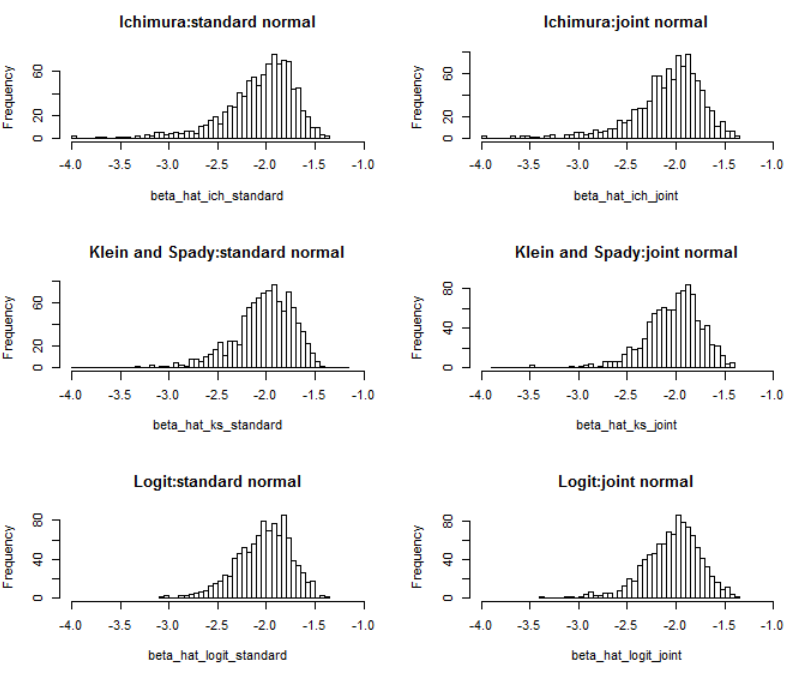
\includegraphics[width=\linewidth]{plot_comparison.png}
 
  \label{fig:plot of estimates}
\end{figure}






\end{document}